\documentclass{article}
\usepackage[a4paper,margin=1.5cm]{geometry}
\usepackage[utf8]{inputenc}

\title{Dynamic labeling}
\author{Elad Noor, Evgeny Onishchenko}

\usepackage{natbib}
\usepackage{graphicx}
\usepackage{amsthm}
\usepackage{amsmath}
\usepackage{amssymb}
\usepackage{mathtools}
\usepackage{hyperref}
\usepackage{pgfplots}

\usepgfplotslibrary{colorbrewer}
\pgfplotsset{cycle list/Set1-8}
\pgfplotsset{compat=1.15}

\newtheorem{theorem}{Theorem}[section]
\newtheorem{corollary}{Corollary}[theorem]
\newtheorem{lemma}[theorem]{Lemma}
\newcommand{\finit}{\ensuremath{\vec{f}^\circ}}
\newcommand{\favg}{\ensuremath{\langle f \rangle}}
\newcommand{\fin}{\ensuremath{\langle f_{\text{in}} \rangle}}
\newcommand{\stot}{\ensuremath{s_\text{tot}}}
\newcommand{\flux}[2]{\ensuremath{v_{{#1} \rightarrow {#2}}}}

\begin{document}

\maketitle

\section{Introduction}

The internal metabolism of cells has always been a tough nut to crack. Spectroscopic methods that can visualize small molecules cover only a handful of specific compounds. On the other hand, the overlapping spectra of the diverse metabolome of most cells makes it extremely difficult to quantify single metabolites using spectroscopic methods. Therefore, the ubiquitous analytical method used in metabolomic studies is mass spectroscopy (MS), which is both specific and sensitive enough to cover most metabolites in the cell. The downsides are, of course, its destructive nature and the required amounts that currently don't allow for single-cells studies of bacteria.

Another complication that makes metabolism difficult to study, is the inconvenient fact that metabolite abundances are usually not the most important phenotype, but rather metabolic flux. Flux is what directs cell resources through different pathways to the target required for cell proliferation (or other factors that affect fitness). Furthermore, the enzymes required to catalyze metabolic reactions are typically more expensive than the intermediates metabolite pools (in terms of dry weight, ATP requirement, maintenance energy, etc.). This means that evolution does not care as much about metabolite abundance as much as enzyme abundance, and therefore would try to reduce unnecessary fluxes as much as possible. A general strategy in Flux Balance Analysis (FBA) for finding a likely flux solution is to minimize the sum of all fluxes. It is, however, way more difficult to measure fluxes compared to metabolite abundances, since flux is an inherently dynamic property and requires a few assumptions and probing techniques to observe in an essentially static and destructive methods such as MS.

Flux measuring methods can be classified into two main categories: steady-state metabolic flux analysis (MFA) and Dynamic Labeling (DL). Both use stable isotopes in order to translate the dynamic flux property into an static property observable by MS. MFA, on the other hand, uses the underlying structures of specific metabolites and detailed atom-mapping networks to follow specific labeled atoms (usually $^{13}$C atoms) and measure their distribution at balanced growth conditions. Then, these patterns are used to infer flux ratios withing central metabolism and reconstruct the flux map. DL is more straightforward, where the cells are perturbed by adding labeled substrates to the medium at time $t = 0$ and following the change in labeling fractions of downstream metabolites. This method is the focus of this work.

In general, DL can be used both in steady-state or perturbed state. Often, the data is used only in a qualitative manner, e.g. to answer which of a set of possible products gets labeled or the timescale required for the labeling to occur. Converting the data to flux is, however, tricky since it also depends on the intermediate metabolite pool sizes and the combinatorics of multiple inputs and outputs to the pathway. To obtain quantitative results, one would require a kinetic model that could simulate the labeling patterns (by ODE integration) and try to fit that to the measured values. The number of unknown parameters in this case is usually much too large and this approach is very rarely applied.

Here, we only discuss the case of steady-state labeling (which means that all fluxes and metabolite abundances are constant, but the labels are not at steady-state). We show that there is a general solution to the ODE system which does not require any of the kinetic parameters, only the fluxes and metabolite pool sizes. In addition, the ODE system can be solved analytically for some specific cases, and for all others by simple numerical tools. We believe that this solution can greatly accelerate the analysis of many dynamic labeling applications and also show how it can help in fitting experimental data.


\section{General solution for dynamic labeling experiments}
Imagine a general metabolic network, which can be described as a standard graph, i.e. all reactions are one-to-one (typically, metabolic networks for medium size or larger will not qualify here, and it would be necessary to use an atom-mapping network for them).

We assume the system is at metabolic steady state, i.e. therefore all fluxes and pool sizes are constant and given by \flux{i}{j} (the flux from $S_i$ to $S_j$) and $s_i$ (the pool size of $S_i$). We define $\flux{i}{j} = 0$. The labeled fractions are not at steady-state and we aim to describe their time evolution, denoted $f_i(t) \equiv s_i^1(t) / (s_i^0(t) + s_i^1(t)) = s_i^1(t) / s_i$. Note that $s_i$ is not a function of time, since it is assumed to be at steady-state. Then:
\begin{eqnarray}
    \frac{d s_i^0}{dt} ~=~
    \sum_j f_j~\flux{j}{i} ~-~ \sum_j f_i~\flux{i}{j} ~=~ 
    \sum_j f_j~\flux{j}{i} ~-~ f_i \sum_j \flux{i}{j}
\end{eqnarray}
which can be written also in matrix notation (where we use the convention that $\vec{x}$ is a row vector):
\begin{eqnarray}
	\frac{d\vec{s}^0}{dt} 
	&=& \vec{f}~\mathbf{V} - \vec{f}~\text{diag}(\mathbf{V}~\vec{1}_n^\top) \\
	\frac{d\vec{f}}{dt}~\text{diag}(\vec{s})
	&=& \vec{f} \left( \mathbf{V} - \text{diag}(\mathbf{V}~\vec{1}_n^\top) \right)
\end{eqnarray}

\subsection{Homogeneous linear system of ODEs}
To summarize the previous section, we showed that dynamic labeling is a homogeneous linear system of ODEs:
\begin{eqnarray}\label{eq:homogenous}
    \frac{d\vec{f}}{d t} &=& \vec{f}~\mathbf{M} \\
    \vec{f}(0) &=& \finit
\end{eqnarray}
where $\mathbf{M} = \left( \mathbf{V} - \text{diag}(\mathbf{V}~\vec{1}_n^\top) \right) \text{diag}(\vec{s})^{-1}$. This system has the general solution:
\begin{eqnarray}
    \vec{f}(t) = \finit~e^{\mathbf{M} t} =  \finit~\mathbf{P}~e^{\mathbf{J}\,t}~\mathbf{P}^{-1}
\end{eqnarray}
where $\mathbf{J}$ is the Jordan normal form of $\mathbf{M}$, i.e. $\mathbf{P}~\mathbf{J}~\mathbf{P}^{-1} = \mathbf{M}$. When $\mathbf{J}$ is a diagonal matrix, $\text{diag}(\vec{\lambda})$, we can change the multiplication order, so that the formula takes on a simpler form $\vec{f}(t) = e^{\vec{\lambda} t}\mathbf{A}$:
\begin{eqnarray}\label{eq:homogenous_solution}
    \vec{f}(t) =
    \finit~\mathbf{P} ~ \text{diag}\left(e^{\vec{\lambda} t}\right) ~ \mathbf{P}^{-1} =
    e^{\vec{\lambda} t} ~ \text{diag}\left(\finit~\mathbf{P}\right) ~ \mathbf{P}^{-1}\,.
\end{eqnarray}

\begin{eqnarray}
\mathbf{M} = \left( \mathbf{V} - \text{diag}(\vec{1}_n~\mathbf{V}) \right) \text{diag}(\vec{s})^{-1}
\end{eqnarray}

\subsection{Average labeling fraction is constant}
The average amount of label in all pools (weighted by their relative sizes) is given by $\favg ~=~ \vec{f} \, \vec{s}^\top / \stot$, where $\stot \equiv \sum_i s_i$. Using the definitions from the previous sections, we can solve the following time derivative:
\begin{eqnarray}
\stot\frac{d\favg}{dt} &=& \frac{d\vec{f}}{dt} \, \vec{s}^\top =
\vec{f} \, \mathbf{M} \, \vec{s}^\top = 
\vec{f} \, \left( \mathbf{V} - \text{diag}(\mathbf{V}~\vec{1}_n^\top) \right) \text{diag}(\vec{s})^{-1} \, \vec{s}^\top \nonumber\\
&=& 
\vec{f} \, \left( \mathbf{V} - \text{diag}(\mathbf{V}~\vec{1}_n^\top) \right) \vec{1}_n^\top =
\vec{f} \, \left( \mathbf{V}~\vec{1}_n^\top - \text{diag}(\mathbf{V}~\vec{1}_n^\top)~\vec{1}_n^\top \right) 
= \vec{f} \, \left( \mathbf{V}~\vec{1}_n^\top - \mathbf{V}~\vec{1}_n^\top \right) = 0
\label{eq:total_label}
\end{eqnarray}
which tells us that $\favg$ is constant, and set by the initial conditions:
\begin{eqnarray}
	\favg &=& \frac{\finit \, \vec{s}^\top}{\stot}
\end{eqnarray}

\subsection{Open systems}
Importantly, our ODE system ignores some fluxes that exist in the metabolic system, but do not have an effect on labeling. This is necessary since a non-trivial steady-state flux requires an open system, where some fluxes enter from the ``outside'' and some material is constantly removed (e.g. to biomass). Also, we will typically want to simulate cases where at some time $t=0$ labels start to spread out from a single node ($S_0$), and it remains fully labeled throughout the experiment. The source of this label (which has to constantly replenish $S_0$) is not included in our system.

Our current definition of $\mathbf{M}$ is only valid for closed systems, and to ...

\subsection{Example: linear pathway with only irreversible steps}
Image a cascade of reactions which is at steady state, but the fluxes are not necessarily equal (e.g. there could be irreversible branching fluxes):
\begin{equation}
    \xrightarrow{v_0} \underset{\downarrow}{S_0} 
    \xrightarrow{v_1} \underset{\downarrow}{S_1} 
    \xrightarrow{v_2} \underset{\downarrow}{S_2}
    \xrightarrow{v_3} \ldots 
    \xrightarrow{v_n} \underset{\downarrow}{S_n}
\end{equation}
At time $t = 0$, the first pool ($S_0$) is replaced with a fully labeled one, while all downstream pools start completely unlabeled. In addition, we define $\tau_i \equiv \frac{s_i}{v_i}$. The system is therefore described by:
\begin{eqnarray}
\finit = \left[1~0~0~\ldots~0\right]
~~~~
\mathbf{M} =
  \begin{bmatrix}
    -1/\tau_0 & 1/\tau_1 & 0 & 0 & \ldots & 0 & 0\\
    0 & -1/\tau_1 & 1/\tau_2 & 0 & \ldots & 0 & 0\\
    0 & 0 & -1/\tau_2 & 1/\tau_3 & \ldots & 0 & 0\\
    0 & 0 & 0 & -1/\tau_3 & \ldots & 0 & 0\\
    & & & \vdots & & &\\
    0 & 0 & 0 & 0 & \ldots & 0 & -1/\tau_n \\
  \end{bmatrix}
\end{eqnarray}

To describe the solution for this ODE system, we first define $\forall i \neq j:~g_{ij} \equiv (1 - \tau_i/\tau_j)^{-1}$, and $\forall i:~g_{ii} \equiv 1$. We use \href{https://www.sympy.org/}{Sympy} to find the Jordan normal form of $\mathbf{M}$
\begin{eqnarray}
\mathbf{J} =
  \begin{bmatrix}
    -\frac{1}{\tau_0} & 0 & 0 & \ldots & 0 \\
    0 & -\frac{1}{\tau_1} & 0 & \ldots & 0 \\
    0 & 0 & -\frac{1}{\tau_2} & \ldots & 0 \\
    0 & 0 & 0 & \ldots & 0 \\
     & \vdots & & & & \\
    0 & 0 & 0 & \ldots & -\frac{1}{\tau_n}
\end{bmatrix}
~~~
\mathbf{P^{-1}} =
\begin{bmatrix}
1 & \prod_1^1 g_{i0} & \prod_1^2 g_{i0} & \prod_1^3 g_{i0} & \prod_1^4 g_{i0} & \ldots & \prod_1^n g_{i0} \\
0 & 1 & \prod_2^2 g_{i1} & \prod_2^3 g_{i1} & \prod_2^4 g_{i1} & \ldots & \prod_2^n g_{i1} \\
0 & 0 & 1 & \prod_3^3 g_{i2} & \prod_3^4 g_{i2} & \ldots & \prod_3^n g_{i2} \\
& \vdots & & & & & \\
0 & 0 & 0 & 0 & 0 & \ldots & 1
\end{bmatrix}
\end{eqnarray}
and\[\finit~\mathbf{P} = \left[1 ~~~ -g_{10}g_{11} ~~~ -g_{20}g_{12}g_{22} ~~~ -g_{30}g_{13}g_{23}g_{33} ~~~ \ldots ~~~ -g_{n0}\prod_{i=1}^n g_{in} \right]\,.\]
Using these values in Equation \ref{eq:homogenous_solution} yields the following expression:
\begin{eqnarray}
	\vec{f}(t) &=& e^{\vec{\lambda} t} ~ \text{diag}\left(\finit~\mathbf{P}\right) ~ \mathbf{P}^{-1} \\
	&=&
	\left[ e^{-\frac{t}{\tau_0}} ~~ e^{-\frac{t}{\tau_1}} ~~ e^{-\frac{t}{\tau_2}} ~~ \ldots ~~ e^{-\frac{t}{\tau_n}}\right]
    \begin{bmatrix}
        1 & \prod_1^1 g_{i0} & \prod_1^2 g_{i0} & \prod_1^3 g_{i0} & \ldots & \prod_1^n g_{i0} \\ \\
        0 & -g_{10}\prod_1^1 g_{i1} & -g_{10}\prod_1^2 g_{i1} & -g_{10}\prod_1^3 g_{i1}  & \ldots & -g_{10}\prod_1^n g_{i1} \\ \\
        0 & 0 & -g_{20}\prod_1^2 g_{i2} & -g_{20}\prod_1^3 g_{i2} & \ldots & -g_{20}\prod_1^n g_{i2} \\
         & \vdots & & & & \\
        0 & 0 & 0 & 0 & \ldots & -g_{n0}\prod_1^n g_{in}
    \end{bmatrix} \nonumber
\end{eqnarray}

We can also write this equation in a compact way without using matrix multiplications:
\begin{eqnarray}
    f_k(t) &=& \left(\prod_{i=1}^{k} g_{i0}\right) e^{- t/\tau_0}
    ~-~ \sum_{j=1}^{k} g_{j0} \left(\prod_{i=1}^{k} g_{ij}\right) e^{- t/\tau_j} \\
    &=& 
    \left(\prod_{i=1}^{k} 1 - \tau_i/\tau_0 \right)^{-1} e^{- t/\tau_0}
    ~-~
    \sum_{j=1}^{k} (1-\tau_j/\tau_0)^{-1} \left(\prod_{i = 1, i \neq j}^{k} 1 - \tau_i/\tau_j\right)^{-1} e^{- t/\tau_j}
\end{eqnarray}

\subsubsection{Defining the internal average labeling fraction}

We define $\fin$ as the weighted average of labels among all internal pools excluding $S_0$, namely 
\begin{eqnarray}
	\fin \equiv 
	\frac{\sum_{i=1}^{n} f_i \, s_i}{\sum_{i=1}^{n} s_i} =
	\frac{\vec{f} \, \vec{s}^\top - f_0 \, s_0}{\stot - s_0} = 
	\frac{\favg \, \stot - f_0 \, s_0}{\stot - s_0}
\end{eqnarray}
This quantity is useful in some experimental setups, where the internal average labeling fraction can be directly measured. For instance, the $^{13}$C fraction of all biomass carbons can be measured by complete oxidation of dry biomass to carbon dioxide (after removing all the externally labeled compounds in the media).

As we showed in Equation \ref{eq:total_label}, $\favg$ is constant and set by the initial conditions. In this case, all pools start unlabeled except for $S_0$ which is fully labeled at $t = 0$, and therefore $\favg = s_0 / \stot$.

\begin{eqnarray}
	\fin &=& 
	\frac{s_0 - f_0 \, s_0}{\stot - s_0} = 
	\frac{1 - f_0}{\stot/s_0 - 1}
\end{eqnarray}


\section{Linear irreversible pathway with dilution}\label{sec:linear_examples}
Assume that the pathway exists inside an exponentially growing cell, all species are at steady state, and that no side fluxes exist besides the growth dilution (which is given by $\mu s_i$). In addition, the final product $S_n$ is a dead-end (e.g. it could be a direct constituent of biomass like a membrane lipid). The fluxes are thus given by:
\begin{equation}
    \flux{i-1}{i} = \mu \sum_{k=i}^n s_k
\end{equation}
and therefore $\tau_i = s_i/v_i = s_i (\mu \sum_{k=i}^n s_k)^{-1}$. It is convenient to define the relative pool size of $S_i$ compared to all the downstream pool (including $S_i$ itself) as $\phi_i \equiv \mu~\tau_i = s_i / \sum_{k=i}^n s_k$. In this case:
\begin{equation}\label{eq:dilution}
    f_k(t) = 1 - \sum_{j=1}^{k} \left(\prod_{i = 1, i \neq j}^{k} 1 - \phi_i/\phi_j\right)^{-1} e^{- \mu t / \phi_j}
\end{equation}

\subsection{Example: four equal pool sizes}
In this example, we choose $n = 4$, $\mu = 1$ hour$^{-1}$ and $s_1 = \ldots = s_4$. Then $\phi_i = 1/(5-i)$ and therefore:
\begin{center}
\begin{tabular}{cccccc}
    $f_1$ = & 1 & $- e^{-4t}$ &&&\\
    $f_2$ = & 1 & $+ 3 e^{-4t}$ & $- 4 e^{-3t}$ &&\\
    $f_3$ = & 1 & $+ 3 e^{-4t}$ & $+ 8 e^{-3t}$ & $- 6 e^{-2t}$ &\\
    $f_4$ = & 1 & $- e^{-4t}$   & $- 4 e^{-3t}$ & $+ 6 e^{-2t}$ & $- 4 e^{-t}$
\end{tabular}
\end{center}

To calculate $f_{tot}$, we can simply average the four fractions:
\begin{equation}
    f_{tot} = \frac{s_1 f_1 + s_2 f_2 + s_3 f_3 + s_4 f_4}{s_1 + s_2 + s_3 + s_4} = \frac{f_1 + f_2 + f_3 + f_4}{4} = 1 - e^{-t}
\end{equation}
which matches our general solution for $f_{tot}$ in equation \ref{eq:ftot}. We can now visualize all four fractions and the average $f_{tot}$:
\begin{center}
	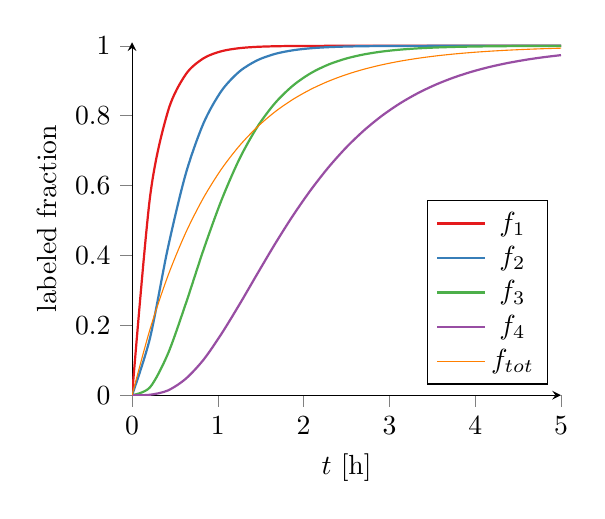
\begin{tikzpicture}
	\begin{axis}[width=200pt,axis x line=bottom, axis y line=left, tick align=outside, domain=0:5, xlabel={$t$ [h]}, ylabel={labeled fraction}, ymin=0, ymax=1.01, legend pos=south east]
    	\addplot+[mark=none,smooth,thick] (\x,{ 1 - exp(-4*\x) });
    	\addlegendentry{$f_1$}
    	\addplot+[mark=none,smooth,thick] (\x,{ 1 + 3*exp(-4*\x) - 4*exp(-3*\x) });
    	\addlegendentry{$f_2$}
    	\addplot+[mark=none,smooth,thick] (\x,{ 1 - 3*exp(-4*\x) + 8*exp(-3*\x) - 6*exp(-2*\x) });
    	\addlegendentry{$f_3$}
    	\addplot+[mark=none,smooth,thick] (\x,{ 1 + 1*exp(-4*\x) - 4*exp(-3*\x) + 6*exp(-2*\x) - 4*exp(-\x) });
    	\addlegendentry{$f_4$}
    	\addplot+[mark=none,smooth] (\x,{ 1 - exp(-\x) });
    	\addlegendentry{$f_{tot}$}
    \end{axis}
	\end{tikzpicture}
\end{center}

\subsection{2-step assembly process with unknown pool sizes}
Here, we consider the most simple case of protein complex assembly. We assume that we can measure the labeling of the prey protein before and after forming a complex with the bait, denoted \textit{precursor pool} and \textit{bound pool} with the corresponding pool sizes ($s_1$ and $s_2$). As before, at time $t = 0$, any newly synthesized protein would be labeled. Additionally, we assume no degradation and irreversible binding. The only diluting factor is the growth rate $\mu$.

So, we can use the general solution from equation \ref{eq:dilution}, where $\phi_1 = s_1 / (s_1 + s_2)$ and $\phi_2 = 1$:
\begin{eqnarray}
    f_1 &=& 1 - e^{- \mu t / \phi_1} \\
    f_2 &=& 1 - \left(1 - 1 / \phi_1 \right)^{-1} e^{- \mu t / \phi_1} - \left(1 - \phi_1 \right)^{-1} e^{- \mu t}
\end{eqnarray}
We can now rewrite $f_2$ as a function of $f_1$ and thus get rid of $t$:
\begin{eqnarray}
    f_2 &=& 1 + \frac{\phi_1}{1-\phi_1} (1 - f_1) - \frac{1}{1-\phi_1} (1 - f_1)^{\phi_1}
\end{eqnarray}
which is a function that looks like this:
\begin{center}
	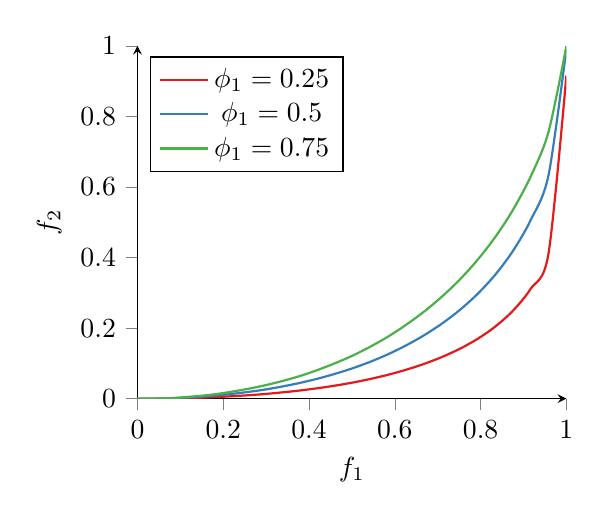
\begin{tikzpicture}[
		declare function={ f2(\x,\y) = 1 + \y/(1-\y)*(1-\x) - 1/(1-\y)*(1-x)^\y ;
		},
	]
	\begin{axis}[width=200pt,axis x line=bottom, axis y line=left, tick align=outside, domain=0:1, xmin=0, xmax=1, xlabel={$f_1$}, ylabel={$f_2$}, ymin=0, ymax=1, legend pos=north west]
    	\addplot+[mark=none,smooth,thick] (\x,{ f2(\x, 0.25) });
    	\addlegendentry{$\phi_1 = 0.25$}
    	\addplot+[mark=none,smooth,thick] (\x,{ f2(\x, 0.5) });
    	\addlegendentry{$\phi_1 = 0.5$}
    	\addplot+[mark=none,smooth,thick] (\x,{ f2(\x, 0.75) });
    	\addlegendentry{$\phi_1 = 0.75$}
	\end{axis}
	\end{tikzpicture}
\end{center}

We can also rewrite the two fraction $f_1$ and $f_2$ as functions of $f_{tot} = 1 - e^{- \mu t}$:
\begin{eqnarray}
    f_1 &=& 1 - (1 - f_{tot})^{1/{\phi_1}} \label{eq:two_step_f1_vs_ftot} \nonumber\\
    f_2 &=& 1 + \frac{\phi_1}{1-\phi_1} (1 - f_{tot})^{1/{\phi_1}} - \frac{1}{1-\phi_1} (1 - f_{tot}) \label{eq:two_step_f2_vs_ftot}
\end{eqnarray}

\begin{center}
	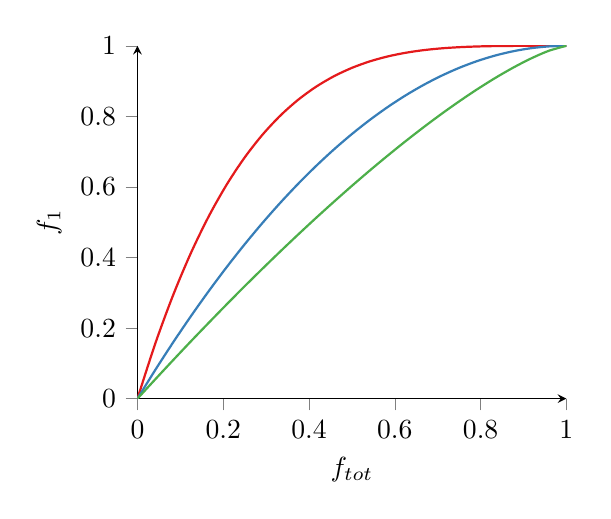
\begin{tikzpicture}[
		declare function={ f1(\x,\y) = 1-(1-\x)^(1/\y) ;
		},
	]
	\begin{axis}[width=200pt,axis x line=bottom, axis y line=left, tick align=outside, domain=0:1, xmin=0, xmax=1, xlabel={$f_{tot}$}, ylabel={$f_1$}, ymin=0, ymax=1, legend pos=south east]
    	\addplot+[mark=none,smooth,thick] (\x,{ f1(\x, 0.25) });
    	\addplot+[mark=none,smooth,thick] (\x,{ f1(\x, 0.5) });
    	\addplot+[mark=none,smooth,thick] (\x,{ f1(\x, 0.75) });
	\end{axis}
	\end{tikzpicture}
	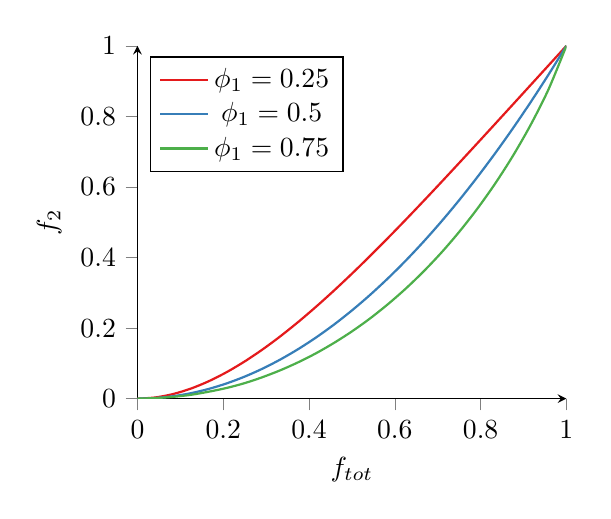
\begin{tikzpicture}[
		declare function={ f2(\x,\y) = 1 + \y/(1-\y)*(1-\x)^(1/\y) - 1/(1-\y)*(1-\x) ;
		},
	]
	\begin{axis}[width=200pt,axis x line=bottom, axis y line=left, tick align=outside, domain=0:1, xmin=0, xmax=1, xlabel={$f_{tot}$}, ylabel={$f_2$}, ymin=0, ymax=1, legend pos=north west]
    	\addplot+[mark=none,smooth,thick] (\x,{ f2(\x, 0.25) });
    	\addlegendentry{$\phi_1 = 0.25$}
    	\addplot+[mark=none,smooth,thick] (\x,{ f2(\x, 0.5) });
    	\addlegendentry{$\phi_1 = 0.5$}
    	\addplot+[mark=none,smooth,thick] (\x,{ f2(\x, 0.75) });
    	\addlegendentry{$\phi_1 = 0.75$}
	\end{axis}
	\end{tikzpicture}
\end{center}

If measuring both $f_1$ and $f_{tot}$ is possible, there is an analytical solution for $\phi_1$:
\begin{eqnarray}
    \phi_1 &=& \frac{\ln(1-f_{tot})}{\ln(1-f_{1})}
\end{eqnarray}
but unfortunately, we can typically only measure $f_2$ and $f_{tot}$, so solving for $\phi_1$ must be done numerically.

\begin{center}
	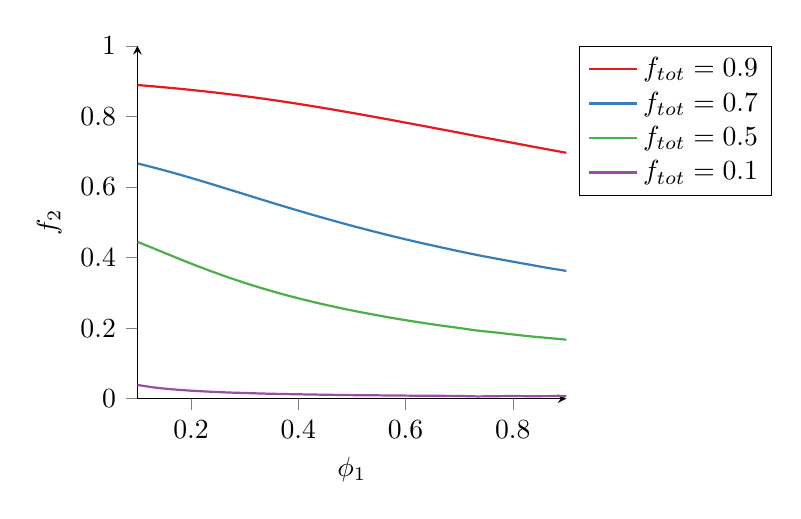
\begin{tikzpicture}[
		declare function={ f2(\x,\y) = 1+\x/(1-\x)*(1-\y)^(1/\x) - 1/(1-\x)*(1-\y);
		},
	]
    \begin{axis}[width=200pt,axis x line=bottom, axis y line=left, tick align=outside, domain=0.1:0.9, xlabel={$\phi_1$}, ylabel={$f_2$}, ymin=0, ymax=1, legend pos=outer north east]
    	\addplot+[mark=none,smooth,thick] (\x,{ f2(\x, 0.9) });
    	\addlegendentry{$f_{tot} = 0.9$}
    	\addplot+[mark=none,smooth,thick] (\x,{ f2(\x, 0.7) });
    	\addlegendentry{$f_{tot} = 0.7$}
    	\addplot+[mark=none,smooth,thick] (\x,{ f2(\x, 0.5) });
    	\addlegendentry{$f_{tot} = 0.5$}
    	\addplot+[mark=none,smooth,thick] (\x,{ f2(\x, 0.1) });
    	\addlegendentry{$f_{tot} = 0.1$}
	\end{axis}
	\end{tikzpicture}
\end{center}


\subsection{3-step assembly process with unknown pool sizes}
Another common case we consider, is similar to the 2-step assembly, except that bound proteins can continue on to an \textit{inaccessible pool} with an unknown size.

So, we can use the general solution from equation \ref{eq:dilution}, where $\phi_1 = s_1 / (s_1 + s_2 + s_3)$, $\phi_2 = s_2 / (s_2 + s_3)$ and $\phi_3 = 1$:
\begin{eqnarray}
    f_1 &=& 1 - e^{- \mu t / \phi_1} \nonumber\\
    f_2 &=& 1 - \left(1 - \phi_2 / \phi_1 \right)^{-1} e^{- \mu t / \phi_1} - \left(1 - \phi_1 / \phi_2 \right)^{-1} e^{- \mu t / \phi_2} \nonumber\\
    f_3 &=& 1 - \left(1 - \phi_2 / \phi_1 \right)^{-1} \left(1 - \phi_3 / \phi_1 \right)^{-1} e^{- \mu t / \phi_1} - \left(1 - \phi_1 / \phi_2 \right)^{-1} \left(1 - \phi_3 / \phi_2 \right)^{-1} e^{- \mu t / \phi_2} - \nonumber\\
    && \left(1 - \phi_1 / \phi_3 \right)^{-1} \left(1 - \phi_2 / \phi_3 \right)^{-1} e^{- \mu t / \phi_3}
\end{eqnarray}

As before, we only care about $f_2$ and $f_{tot}$ since they are measurable, so we express one as a function of the other:
\begin{eqnarray}
    f_{tot} &=& 1 - e^{- \mu t}\nonumber\\
    f_2 &=& 1 + \frac{\phi_1}{\phi_2 - \phi_1} (1 - f_{tot})^{1/{\phi_1}} - \frac{\phi_2}{\phi_2-\phi_1} (1 - f_{tot})^{1/{\phi_2}} \label{eq:three_step_f2}
\end{eqnarray}

Importantly, there is a complete symmetry between $\phi_1$ and $\phi_2$ (i.e. $f_2(\phi_1, \phi_2) = f_2(\phi_2, \phi_1)$, and that means that if we use this function to fit experimental data, we would not be able to distinguish between two equivalent solutions ($\phi_1$, $\phi_2$) and ($\phi_2$, $\phi_1$).

The effect of a large inaccessible pool (small $\phi_2$) is to shift the curves to the left (i.e. make the labeling of $f_2$ occur at earlier and at lower levels of $f_{tot}$), as seen in the following example:
\begin{center}
	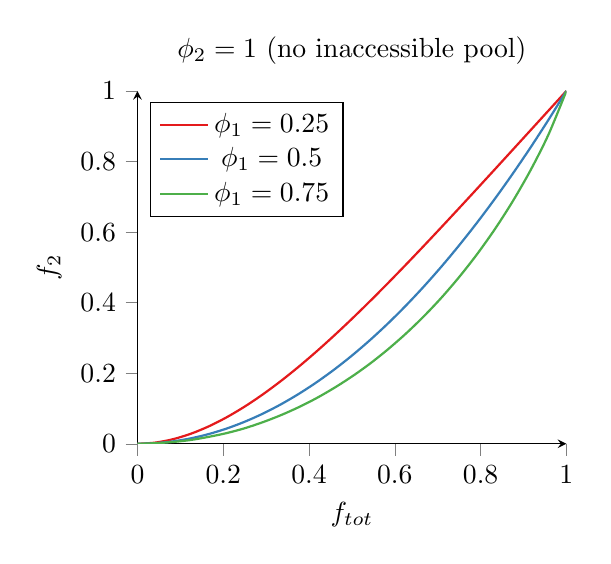
\begin{tikzpicture}[
		declare function={ f2(\x,\y,\z) = 1 + \y/(\z - \y)*(1-\x)^(1/\y) - \z/(\z - \y)*(1-\x)^(1/\z);
		},
	]
	\begin{axis}[title={$\phi_2 = 1$ (no inaccessible pool)}, width=200pt,axis x line=bottom, axis y line=left, tick align=outside, domain=0:1, xlabel={$f_{tot}$}, ylabel={$f_2$}, ymin=0, ymax=1, legend pos=north west]
    	\addplot+[mark=none,smooth,thick] (\x,{ f2(\x, 0.25, 1) });
		\addlegendentry{$\phi_1 = 0.25$}
		\addplot+[mark=none,smooth,thick] (\x,{ f2(\x, 0.5, 1) });
		\addlegendentry{$\phi_1 = 0.5$}
		\addplot+[mark=none,smooth,thick] (\x,{ f2(\x, 0.75, 1) });
		\addlegendentry{$\phi_1 = 0.75$}
	\end{axis}
	\end{tikzpicture}
	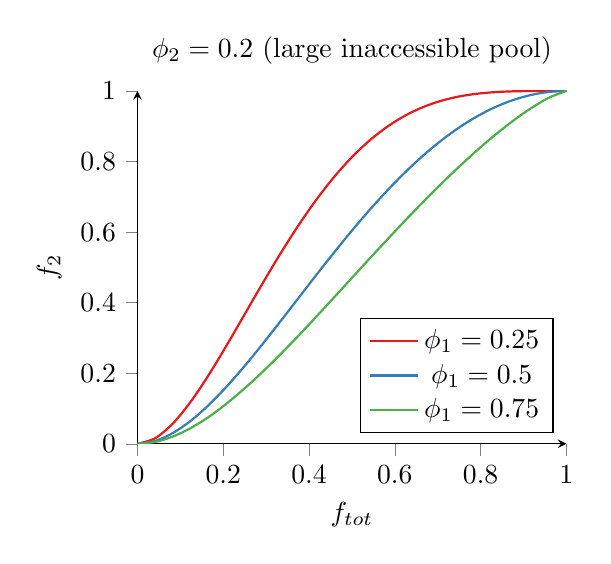
\begin{tikzpicture}[
		declare function={ f2(\x,\y,\z) = 1 + \y/(\z - \y)*(1-\x)^(1/\y) - \z/(\z - \y)*(1-\x)^(1/\z);
		},
	]
	\begin{axis}[title={$\phi_2 = 0.2$ (large inaccessible pool)}, width=200pt,axis x line=bottom, axis y line=left, tick align=outside, domain=0:1, xlabel={$f_{tot}$}, ylabel={$f_2$}, ymin=0, ymax=1, legend pos=south east]
    	\addplot+[mark=none,smooth,thick] (\x,{ f2(\x, 0.25, 0.2) });
		\addlegendentry{$\phi_1 = 0.25$}
    	\addplot+[mark=none,smooth,thick] (\x,{ f2(\x, 0.5, 0.2) });
    	\addlegendentry{$\phi_1 = 0.5$}
    	\addplot+[mark=none,smooth,thick] (\x,{ f2(\x, 0.75, 0.2) });
    	\addlegendentry{$\phi_1 = 0.75$}
	\end{axis}
	\end{tikzpicture}
\end{center}
As expected, the figure on the left ($\phi_2 = 1$) is identical to the one in the previous section (2-step model). We can conclude that $f_2$ decreases with $\phi_1$ as well as $\phi_2$.

\subsection{Solution for the limit of equal \texorpdfstring{$\phi$}{phi} values}
The function in equation \ref{eq:three_step_f2} is not defined for $\phi_1 = \phi_2$ (since we have a 0 divided by 0 situation). However, we can solve the limit using L'H\^{o}pital's rule (we assume $\phi_1$ is constant and derive the numerator and denominator according to $\phi_2$):
\begin{eqnarray}
	f_2 &=& 
	\frac{\phi_2 - \phi_1 + \phi_1 (1-f_{tot})^{1/{\phi_1}} - \phi_2 (1-f_{tot})^{1/{\phi_2}}}{\phi_2 - \phi_1}
	\nonumber\\
	&=& \frac{1 - (1-f_{tot})^{1/{\phi_2}} + \phi_2 \cdot \phi_2^{-2} \cdot \ln{(1-f_{tot})} \cdot(1-f_{tot})^{1/{\phi_2}}}{1}
	\nonumber\\
	&=& 1 - \left(1 - \frac{\ln{(1-f_{tot})}}{\phi_2} \right) \cdot (1-f_{tot})^{1/{\phi_2}}
\end{eqnarray}
where we used the formula $\frac{\partial a^{f(x)}}{\partial x} = \frac{\partial f}{\partial x}\ln(a) a^{f(x)}$. This is what this function looks like for several values of $\phi_1 = \phi_2 = \phi$:
\begin{center}
	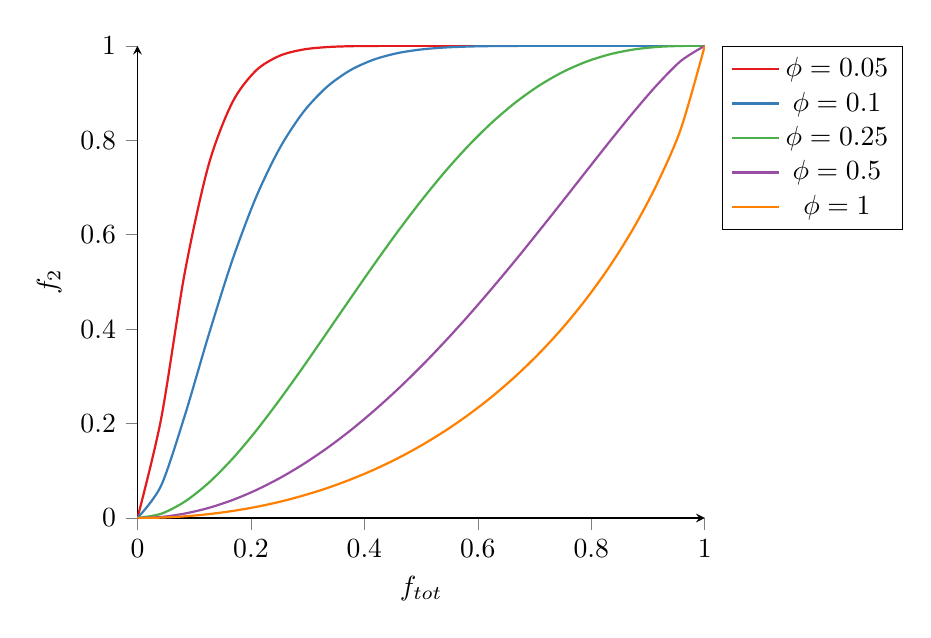
\begin{tikzpicture}[
		declare function={ f2app(\x,\y) = 1 - (1 - ln(1-\x) / \y) * (1-\x) ^ (1/\y);
		},
	]
	\begin{axis}[width=250pt,axis x line=bottom, axis y line=left, tick align=outside, domain=0:1, xmin=0, xmax=1, xlabel={$f_{tot}$}, ylabel={$f_2$}, ymin=0, ymax=1, legend pos=outer north east]
	\addplot+[mark=none,smooth,thick] (\x,{ f2app(\x, 0.05) });
	\addlegendentry{$\phi = 0.05$}
	\addplot+[mark=none,smooth,thick] (\x,{ f2app(\x, 0.1) });
	\addlegendentry{$\phi = 0.1$}
	\addplot+[mark=none,smooth,thick] (\x,{ f2app(\x, 0.3) });
	\addlegendentry{$\phi = 0.25$}
	\addplot+[mark=none,smooth,thick] (\x,{ f2app(\x, 0.6) });
	\addlegendentry{$\phi = 0.5$}
	\addplot+[mark=none,smooth,thick] (\x,{ f2app(\x, 1) });
	\addlegendentry{$\phi = 1$}
	\end{axis}
	\end{tikzpicture}
\end{center}

\subsection{Observability of \texorpdfstring{$\phi_1$}{phi1} and \texorpdfstring{$\phi_2$}{phi2}}
It is noteworthy, that even though $f_2$ has two degrees of freedom ($\phi_1$ and $\phi_2$), the function is \textit{almost} redundant in parameter space, meaning that the shape of $f_2$ is almost constant if $\phi_1 \cdot \phi_2 =$ const. Below is an example for a range of values, where $\phi_1 \cdot \phi_2 = 0.36$. We also compare that to the limit $\phi_1 = \phi_2 = 0.6$.

\begin{center}
	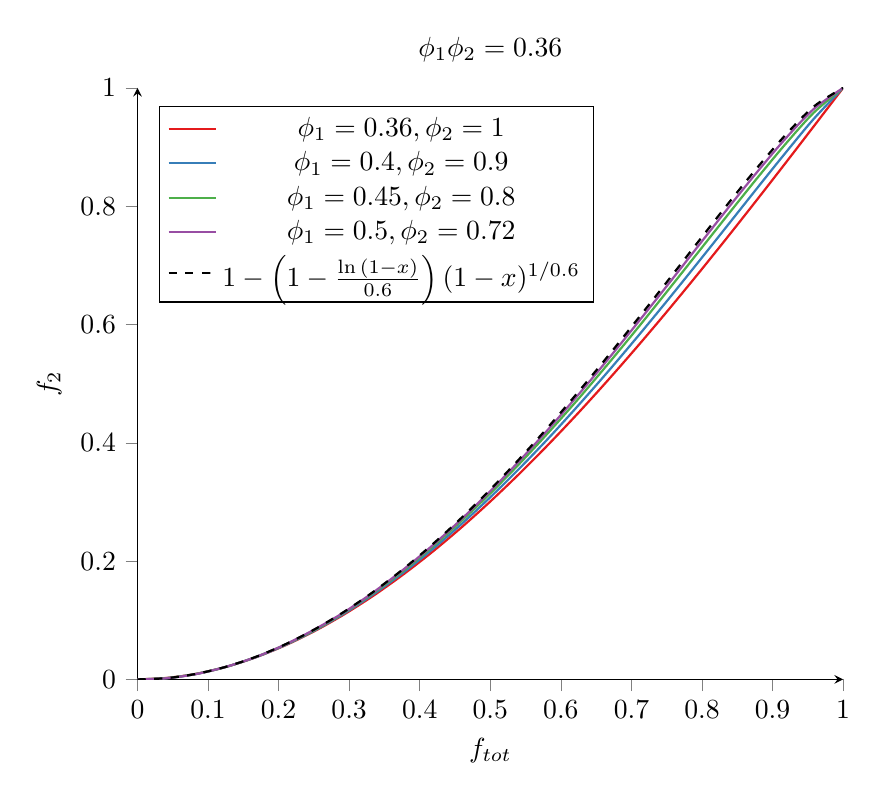
\begin{tikzpicture}[
	declare function={ f2(\x,\y,\z) = 1 + \y/(\z - \y)*(1-\x)^(1/\y) - \z/(\z - \y)*(1-\x)^(1/\z);
	},
	declare function={ f2app(\x,\y) = 1 - (1 - ln(1-\x) / \y) * (1-\x) ^ (1/\y);
	},
	]
	\begin{axis}[title={$\phi_1 \phi_2 = 0.36$}, width=300pt,axis x line=bottom, axis y line=left, tick align=outside, domain=0:1, xlabel={$f_{tot}$}, ylabel={$f_2$}, ymin=0, ymax=1, legend pos=north west]
		\addplot+[mark=none,smooth,thick] (\x,{ f2(\x, 0.36, 1) });
		\addlegendentry{$\phi_1 = 0.36, \phi_2 = 1$}
		\addplot+[mark=none,smooth,thick] (\x,{ f2(\x, 0.4, 0.9) });
		\addlegendentry{$\phi_1 = 0.4, \phi_2 = 0.9$}
		\addplot+[mark=none,smooth,thick] (\x,{ f2(\x, 0.45, 0.8) });
		\addlegendentry{$\phi_1 = 0.45, \phi_2 = 0.8$}
		\addplot+[mark=none,smooth,thick] (\x,{ f2(\x, 0.5, 0.72) });
		\addlegendentry{$\phi_1 = 0.5, \phi_2 = 0.72$}
		\addplot+[color=black,dashed,mark=none,smooth,thick] (\x,{ f2app(\x, 0.6) });
		\addlegendentry{$1 - \left(1 - \frac{\ln{(1 - x)}}{0.6} \right) (1 - x)^{1/{0.6} }$}
	\end{axis}
	\end{tikzpicture}
\end{center}

This means, that if we try to fit these parameters to measured data, we might not be able to distinguish between a set of nearly equivalent solutions (with the same $\phi_1 \cdot \phi_2$ value).

\subsubsection{Example with pool size as parameters}
Given two scenarios, where the pool size ratios are 4:3:3 and 5:2:3, the $f_2$ trajectory will look exactly the same.

\begin{center}
	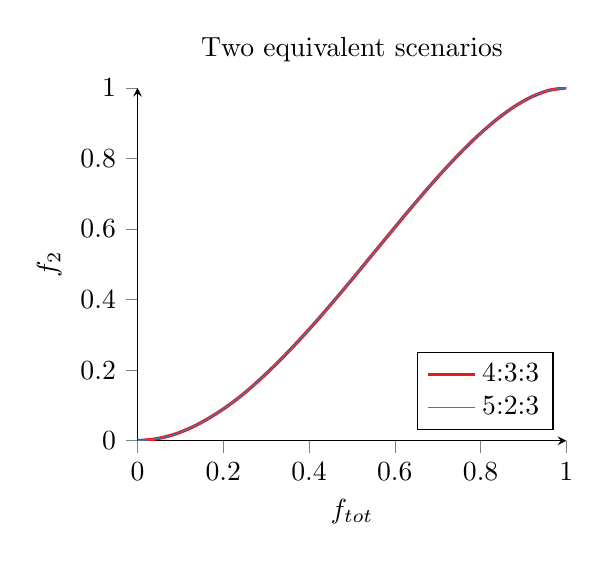
\begin{tikzpicture}[
	declare function={ f2(\x,\y,\z) = 1 + \y/(\z - \y)*(1-\x)^(1/\y) - \z/(\z - \y)*(1-\x)^(1/\z);
	},
	]
	\begin{axis}[title={Two equivalent scenarios}, width=200pt,axis x line=bottom, axis y line=left, tick align=outside, domain=0:1, xlabel={$f_{tot}$}, ylabel={$f_2$}, ymin=0, ymax=1, legend pos=south east]
	\addplot+[mark=none,smooth,very thick] (\x,{ f2(\x, 0.4, 0.5) });
	\addlegendentry{4:3:3}
	\addplot+[mark=none,smooth] (\x,{ f2(\x, 0.5, 0.4) });
	\addlegendentry{5:2:3}
	\end{axis}
	\end{tikzpicture}
\end{center}

\section{Linear reversible pathway with dilution}
In this section, we relax our assumption that all reactions are irreversible, but keep focusing on linear pathways whose fluxes are determined by dilution. Unfortunately, the solution for general pathway lengths is extremely complex. Therefore, the only analytical solution we will discuss here is the case of $n = 2$.

\subsection{2-step assembly with reversibility}

\begin{equation}
    \rightarrow S_0 
    \rightarrow \underset{\downarrow}{S_1}
    \rightleftarrows \underset{\downarrow}{S_2}
\end{equation}
As usual, we assume that the system is at balanced growth, so that the dilution fluxes are proportional to their pool sizes, i.e. $\mu s_i$. So:
\begin{eqnarray}
    \flux{1}{2} &=& \mu s_2 + \flux{2}{1}\\
    \flux{0}{1} &=& \mu (s_1 + s_2)
\end{eqnarray}

For simplicity, we define $x \equiv \flux{2}{1} / (\mu s_2)$, therefore:
\[\mathbf{V} =
    \begin{bmatrix}
        0 & \mu (s_1 + s_2) & 0\\
        0 & 0 & \mu s_2 (1 + x) \\
        0 & \mu s_2 x & 0 \\
        0 & 0 & 0 \\
    \end{bmatrix}
\]

The we use the formula $\mathbf{M} = \text{diag}(\vec{s})^{-1} \cdot \left( \mathbf{V}^\top - \text{diag}(\mathbf{V}^\top~\vec{1}_n) \right)$ to get

\[
\mathbf{M} = \mu \cdot 
    \begin{bmatrix}
        0 & 0 & 0  \\
        1 + s_2/s_1 & - 1 - (1+x) s_2 / s_1 & x s_2 / s_1 \\
        0 & 1+x  & -1-x
    \end{bmatrix}
\]
As before, we can reduce the number of parameters by setting $\phi_1 \equiv \frac{s_1}{s_1+s_2}$:
\[
\mathbf{M} = \mu \cdot 
    \begin{bmatrix}
        0 & 0 & 0  \\
        1/\phi_1 & - 1 - (1+x)(1/\phi_1-1) & x (1/\phi_1-1) \\
        0 & 1+x  & -1-x
    \end{bmatrix}
\]
and then find the Jordan normal form for $\mathbf{M}$ using \href{https://www.sympy.org/}{Sympy} while solving for $\mathbf{P}~\text{diag}\left(\mathbf{P}^{-1} ~\finit\right)$:
\begin{eqnarray}
\mathbf{J} = \mu \cdot
  \begin{bmatrix}
    0 & 0 & 0 \\
    0 & -\frac{x+1}{\phi_1} & 0 \\
    0 & 0 & -1
\end{bmatrix}
~~~~
\mathbf{P}~\text{diag}\left(\mathbf{P}^{-1} ~\finit\right) =
    \begin{bmatrix}
        1 & 0 & 0 \\
        1 & \frac{\phi_1 - 1}{x + 1 - \phi_1} & -\frac{x}{x + 1 - \phi_1} \\
        1 & \frac{\phi_1}{x + 1 - \phi_1} & -\frac{x+1}{x + 1 - \phi_1} 
    \end{bmatrix}
\end{eqnarray}
We can continue to simplify this expression by defining $\phi_1' \equiv \phi_1/(1+x)$ and get the following:
\begin{eqnarray}
    f(t) = \mathbf{P}~\text{diag}\left(\mathbf{P}^{-1} ~\finit\right) \cdot e^{\mathbf{J}t} = 
    \begin{bmatrix}
        1 & 0 & 0 \\
        1 & \frac{\bar{\phi}_1 - 1/(1+x)}{1 - \phi_1'} & -\frac{x/(1+x)}{1 - \phi_1'} \\
        1 & \frac{\phi_1'}{1 - \phi_1'} & -\frac{1}{1 - \phi_1'}
    \end{bmatrix} \cdot 
    \begin{bmatrix}
        1 \\
        e^{-\mu\,t / \phi_1'} \\
        e^{-\mu\,t}
    \end{bmatrix}
\end{eqnarray}

And focusing only on $f_2(t)$ we get this final expression
\begin{eqnarray}
    f_2 ~=~ 1 + \frac{\phi_1'}{1 - \phi_1'} (1-f_{tot})^{1/\phi_1'} ~-~ \frac{1}{1 - \phi_1'} (1-f_{tot})
\end{eqnarray}
where again we substituted $e^{\mu\,t}$ with $1-f_{tot}$.

This equation is completely identical to the solution for $f_2$ in the 2-step irreversible model (Equation \ref{eq:two_step_f2_vs_ftot}), where $\phi_1'$ replaces $\phi_1$. That means that for any $x > 0$, we will be able to fit $f_2$ as a function of $f_{tot}$ precisely also with an irreversible model, and the precursor pool $\phi_1$ will be underestimated by a factor of $1+x$.

\subsection{Analytical solution for maturation time}
We define the maturation time $t_{1/2}$ as the time after which a protein that starts in $S_1$ to have a 50\% chance of reaching $S_2$. 

In the 2-step reversible model, the total flux from $S_1$ to $S_2$ is $\mu s_2 (1+x)$, and therefore the chance of any molecule in $S_1$ to make the transition in a short time interval $dt$ is $\mu s_2/s_1 (1+x) dt$. We can replace $s_2/s_1$ with $1/\phi_1 - 1$.

We denote by $P(t)$, the probability that our protein of interest has moved to $S_2$ (matured) before time $t$. The chance of making the transition exactly between $t$ and $t+dt$ is the probability it did not happen already before $t$ (which is $1 - P(t)$) times the probability we just calculated earlier:
\begin{eqnarray}
    dP &=& P(t + dt) - P(t) = \left(1 - P(t)\right) \mu s_2/s_1 (1+x) dt \\
    \int_0^T \frac{1}{1-P} dP &=& \int_0^T s_2/s_1 \mu (1+x)~dt  \\
    -\ln(1-P) &=& s_2/s_1 \mu (1+x)t = (1/\phi_1 - 1)\mu (1+x)t  \\
    t &=& \frac{-\ln(1-P(t))}{\mu (1+x)} \frac{\phi_1}{1 - \phi_1}\,.
\end{eqnarray}

Now, imagine that we fit the precursor pools using data while assuming that the reactions are irreversible. In this case, we are going to underestimate $\phi_1$ by a factor of $(1+x)$, when trying to estimate $t$. To understand how this assumption affects the result, we define our new estimate as:
\begin{eqnarray}
    t' &\equiv& \frac{-\ln(1-P)}{\mu} \cdot \frac{\phi'_1}{1 - \phi'_1} 
    = \frac{-\ln(1-P)}{\mu} \cdot \frac{\phi_1/(1+x)}{1 - \phi_1/(1+x)} \nonumber\\
    &=& \frac{-\ln(1-P)}{\mu (1+x)} \cdot \frac{\phi_1}{1 - \phi_1/(1+x)} 
    = t \cdot \frac{1 - \phi_1}{1 - \phi_1/(1+x)}
\end{eqnarray}
and therefore
\begin{eqnarray}
    1 ~\geq~ \frac{t'}{t} ~>~ 1-\phi_1
\end{eqnarray}
or in other words, if we use an irreversible model to find the maturation, we might underestimate it, but not by more than a factor of $1-\phi_1$.

\clearpage
\section{Fitting measured data}

\subsection{Using the 2-step model}
The common scenario would be that $\tau_i$ are unknown, and we have several time point measurements of some or all $f_i$. In this example, we assume again a 3-step chain, where we measure $f_{tot}$ and $f_2$, and the free parameters are $\phi_1$ and $\phi_2$. 

\subsection{How to infer fluxes from labeling data}

We assume that the data was generated from a system such as in equation \ref{eq:homogenous}, with a diagonalizable matrix $\mathbf{M}$. Then, we can fit our data (which is $\vec{f}$ measured at multiple time points) using the formula $\vec{f}(t) = \mathbf{A} e^{\vec{\lambda} t}$. Then, from equation \ref{eq:homogenous_solution} we know that $\mathbf{P} = \mathbf{A} \mathbf{D}^{-1}$, where $\mathbf{D}$ is some fully ranked diagonal matrix. Even though $\mathbf{D}$ is somehow dependent on $\mathbf{P}$ and $\mathbf{A}$, it wouldn't matter for finding $\mathbf{M}$, since:
\begin{eqnarray}
    \mathbf{M} = \mathbf{P}~\text{diag}(\vec{\lambda})~\mathbf{P}^{-1} = \mathbf{A}\mathbf{D}^{-1}~\text{diag}(\vec{\lambda})~\mathbf{D}\mathbf{A}^{-1} = 
    \mathbf{A}\mathbf{D}^{-1}\mathbf{D}~\text{diag}(\vec{\lambda})~\mathbf{A}^{-1} = 
    \mathbf{A}~\text{diag}(\vec{\lambda})~\mathbf{A}^{-1}
\end{eqnarray}
where $\text{diag}(\vec{\lambda})~\mathbf{D} = \mathbf{D}~\text{diag}(\vec{\lambda})$ since they are both diagonal matrices. Therefore, we can simply ignore the $\mathbf{D}$ matrix altogether, and use the solution:
\begin{eqnarray}
    \mathbf{\bar{V}} = \mathbf{M}^\top~\text{diag}(\vec{s}) = \left(\mathbf{A}~\text{diag}(\vec{\lambda})~\mathbf{A}^{-1} \right)^\top~\text{diag}(\vec{s})
\end{eqnarray}
where $\mathbf{\bar{V}} = \mathbf{V} - \text{diag}(\vec{1}_n~\mathbf{V})$, i.e. the fluxes would be the off-diagonal values of $\mathbf{\bar{V}}$.

\end{document}